\documentclass[conference]{IEEEtran}
\IEEEoverridecommandlockouts
%Template version as of 6/27/2024

\usepackage{cite}
\usepackage{amsmath,amssymb,amsfonts}
\usepackage{algorithmic}
\usepackage{graphicx}
\usepackage{textcomp}
\usepackage{xcolor}
\usepackage{array}
\usepackage{booktabs}
\usepackage{url}

% A rule between every data row costs height, and the paper is capped at six
% pages. Trimming booktabs' default separation (0.4ex/0.65ex) keeps the rules
% visibly open while buying back the space the extra ~30 of them consume.
\setlength{\aboverulesep}{0.25ex}
\setlength{\belowrulesep}{0.35ex}

% Justified table notes. The width has to be the tabular's own, so the tabular is
% typeset into a box first and measured: a note set to \columnwidth would overhang
% a narrower table, and a note hand wrapped into \multicolumn rows cannot justify
% at all, which is what these two notes did before.
\newsavebox{\tablebox}
\newcommand{\tablenote}[1]{%
  \par\vspace{2pt}%
  \parbox{\wd\tablebox}{\footnotesize #1\par}}
% hyperref last: makes \cite, \ref and URLs clickable
\usepackage[hidelinks,breaklinks=true]{hyperref}

\newcommand{\ugm}{$\mu$g\,m$^{-3}$}

% Table captions on one centred line, "TABLE I: Text", roman rather than small
% caps. This is IEEEtran's own \@makecaption with the table branch rewritten and
% the figure branch copied verbatim, so figures keep the house format and the
% caption package -- which warns that it does not know this class -- stays out.
\makeatletter
\long\def\@makecaption#1#2{%
\ifx\@captype\@IEEEtablestring
  \footnotesize\bgroup\par\centering\@IEEEtabletopskipstrut
  \setbox\@tempboxa\hbox{\normalfont\footnotesize #1: #2}%
  \ifdim\wd\@tempboxa>\hsize
    \parbox[t]{\hsize}{\normalfont\footnotesize\centering #1: #2\par}%
  \else
    \box\@tempboxa
  \fi
  \par\addvspace{0.5\baselineskip}\egroup
  \@IEEEtablecaptionsepspace
\else
  \@IEEEfigurecaptionsepspace
  \setbox\@tempboxa\hbox{\normalfont\footnotesize {#1.}\nobreakspace\nobreakspace #2}%
  \ifdim\wd\@tempboxa>\hsize
    \setbox\@tempboxa\hbox{\normalfont\footnotesize {#1.}\nobreakspace\nobreakspace}%
    \parbox[t]{\hsize}{\normalfont\footnotesize\noindent\unhbox\@tempboxa#2}%
  \else
    \ifCLASSOPTIONconference \hbox to\hsize{\normalfont\footnotesize\hfil\box\@tempboxa\hfil}%
    \else \hbox to\hsize{\normalfont\footnotesize\box\@tempboxa\hfil}%
    \fi
  \fi
\fi}
\makeatother

\begin{document}

\title{Quantifying the Cost of Monitoring Record Fragmentation in Short Horizon PM\textsubscript{2.5} Forecasting
}

% \author{\IEEEauthorblockN{Tanvir Anjum Apurbo}
% \IEEEauthorblockA{\textit{Dept. of Computer Science and Eng.} \\
% \textit{Southeast University}\\
% Tejgaon, Dhaka-1208, Bangladesh \\
% anjumtanvir667@gmail.com}
% }

\maketitle

\begin{abstract}
Short horizon PM\textsubscript{2.5} forecasting is benchmarked almost entirely on accuracy, on
records whose gaps are treated as a preprocessing detail. This paper asks whether the
fragmentation of the monitoring record, rather than the model class, decides which method wins.
Nine years of hourly observations from Dhaka (82.3 per cent hourly coverage) are fused with
reanalysis meteorology into 102 predictors, and compact sequence models under a 100{,}000
parameter budget are compared against tree ensembles, linear models and the classical baselines
air quality work often omits, at five horizons. At 24 hours the validation selected recurrent
model attains an RMSE of 57.70 \ugm{} against 58.50 for the best classical competitor, with a
Holm adjusted Diebold and Mariano $p$ of 0.037, yet a 95 per cent model confidence set retains
five of nine candidates, so the finding is about tiers and not architectures. A controlled gap
injection experiment then degrades a near complete record two ways that remove identical hour
counts and differ only in arrangement. The sequence tier loses 0.0394 skill to arrangement
alone (50 matched pairs, Holm $p<0.0001$), the only family whose loss is significant on all
three donor stations. Because a scored row needs unbroken history, a gap costs the hours it
removes plus the backward reach behind them. Shortening that reach from 192 to 48 hours removes
97 per cent of the penalty, and a closed form for usable rows fitted on 101 cells predicts 404
held out cells at $R^2=0.982$. Availability is therefore reported as a first class metric, since
the configured reach answers only 76.4 per cent of test hours and shortening it costs no
measurable accuracy.
\end{abstract}

\begin{IEEEkeywords}
air quality forecasting, PM\textsubscript{2.5}, missing data, record fragmentation,
recurrent neural networks, forecast availability, model confidence set
\end{IEEEkeywords}

\section{Introduction}

Fine particulate matter is the environmental exposure most closely tied to premature
mortality worldwide, and the World Health Organization guideline value is exceeded across
most of South Asia for most of the year \cite{who2021}. Dhaka is among the cities where a
credible next day forecast would carry immediate public health value, and also among those
where the observational record needed to build one is thinnest. Those two facts are usually
treated as independent. They are not.

A decade of data driven air quality forecasting has converged on a familiar protocol. A series
is obtained, absences are filled by interpolation or a nearest neighbour rule, a deep
architecture is trained, and the error is compared against a small set of competitors
\cite{li2017lstm, karnati2025}. Missingness enters this protocol once, as a preprocessing
decision, and leaves it as a sentence in the methods section. The literature treating
missingness as a modelling object rather than a nuisance sits largely in clinical time series
\cite{che2018grud}. What has not been asked, to our knowledge, is the prior question. If two
records differ in how their absences are arranged, does the arrangement alone change which
method a benchmark recommends?

The question cannot be settled by comparing cities, because two records drawn from different
places differ in climate, instrument, span, pollution regime and continuity at once, so a
ranking that moves between them is attributable to everything at once. What is needed is a
counterfactual on a single record. This paper builds one. We assemble a leakage controlled
pipeline over nine years of hourly PM\textsubscript{2.5} from Dhaka fused with reanalysis
meteorology, benchmark three tiers of method at five horizons, and then hold the record fixed
while manipulating only the arrangement of its absences. Fig.~\ref{fig:arch} shows the design.

\begin{enumerate}
\item \textbf{A controlled gap injection experiment} in which two arms remove identical hour
counts and differ only in contiguity. Arrangement alone costs the sequence tier 0.0394 skill,
the only family significant on all three donor stations.
\item \textbf{A mechanism, fixed by design rather than by regression.} A scored row needs
unbroken history over a sterilisation radius, and shortening it from 192 to 48 hours removes
97 per cent of the penalty.
\item \textbf{A closed form for usable supervision}, fitted on 101 cells and predicting 404
held out cells at $R^2=0.982$ across two further stations and a quartered radius.
\item \textbf{Forecast availability as a reported quantity}, with a decision rule for the
backward reach that needs only run lengths and costs nothing to evaluate.
\end{enumerate}

\begin{figure*}[!t]
\centerline{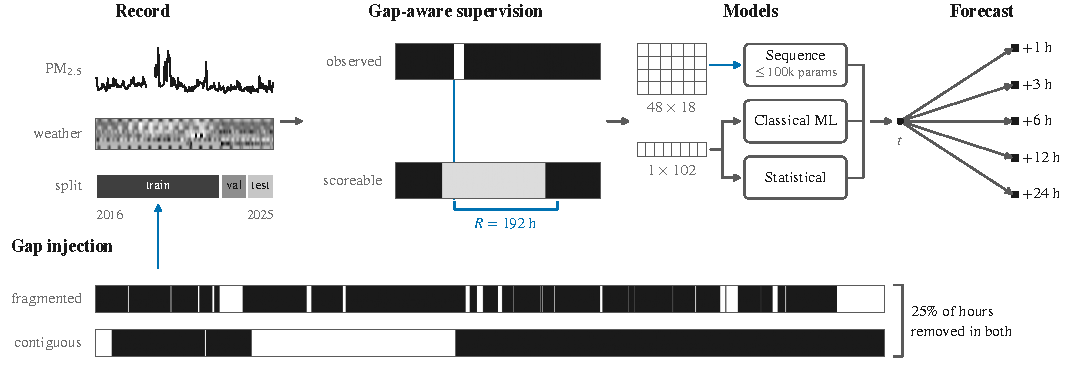
\includegraphics[width=\linewidth]{fig00_architecture.pdf}}
\caption{Study design. A scored row requires unbroken history over a sterilisation radius
$R$, drawn at the configured $R=192$~h. Tabular models receive 102 engineered predictors per
row; the sequence tier receives 18 contemporaneous channels over a window, because engineered
history features restate what the window already contains. The lower panel shows the two
injection arms, which remove the same number of observed hours and differ only in arrangement.}
\label{fig:arch}
\end{figure*}

\section{Related Work}

Recurrent architectures entered air quality forecasting by direct transfer from sequence
modelling \cite{hochreiter1997lstm, cho2014gru}, and the canonical demonstration on pollutant
concentrations reports gains over feedforward and statistical competitors \cite{li2017lstm}.
Subsequent work has broadened the architecture space without broadening the comparison much.
Recent evidence that a single linear layer matches or exceeds transformer forecasters
\cite{zeng2023dlinear} makes the choice of baseline, rather than of architecture, the load
bearing decision, so both linear models enter here as first class competitors.

Missing data in air quality series is normally addressed as imputation, and comparative studies
conclude by recommending one \cite{karnati2025}. That framing assumes filled values restore the
record, and under the classical taxonomy \cite{rubin1976} the assumption concerns the mechanism
generating absence. Our concern is downstream of it. Even when every filled value is correct, a
supervised row built from a window of history is unavailable whenever that window straddles a
gap, so absences impose a structural cost no imputation policy removes. Work on recurrent
models with informative missingness \cite{che2018grud} shares the intuition but treats the
pattern as a signal to exploit rather than a budget to spend.

The statistical apparatus for comparing forecasters is meanwhile mature and underused here.
Pairwise accuracy tests \cite{diebold1995}, familywise error control \cite{holm1979}, the
model confidence set \cite{hansen2011mcs} and block resampling for dependent errors
\cite{kunsch1989} are all standard, and their absence is why a table of closely spaced errors
is read as a ranking.

\section{Study Design}

\subsection{Records and predictors}

The primary target is hourly PM\textsubscript{2.5} from the United States Embassy monitor in
Dhaka, retrieved from the OpenAQ archive \cite{openaq}, spanning 2016 to 2025. Of the
79{,}216 hours in that span, 65{,}214 are observed, giving 82.3 per cent coverage over 7.44
usable years, broken by 2{,}074 distinct gaps of which 1{,}324 last a single hour and the
longest runs 2{,}712 hours. The distribution is severe, with a mean of 93.7 \ugm{} and half
of all hours above the Bangladesh 24 hour standard of 65 \ugm{} \cite{doe2025}.
Meteorological drivers come from NASA POWER hourly point reanalysis \cite{nasapower}. A
second record, the Beijing multi site archive \cite{zhang2017beijing}, supplies both the
cross city comparison and the donor stations for the injection experiment.

Feature construction yields 102 predictors covering lagged concentrations, rolling statistics,
meteorological history and calendar terms. The sequence tier does not receive them. It receives
18 contemporaneous channels over a window, because a lag feature at time $t$ is by construction
the same channel at $t$ minus the lag, already inside the window. Supplying both produced a
collinear input and handicapped the tier against competitors those columns help.

\subsection{Scored rows and the sterilisation radius}

Five rules are enforced structurally rather than by convention. Meteorology is never read
beyond the forecast origin. Splits are chronological and scalers are fitted on training data
only. Imputation never crosses a split boundary and is limited to a short backward fill. Any
window whose internal timestamps are not contiguous is rejected and counted. Each horizon is
forecast directly by its own model rather than by recursive rollout.

The fourth rule organises the rest of this paper. A row at time $t$ is scored only if it
carries unbroken observed history back to $t-L$ and an observed target at $t+h$ in the same
run. Writing $W$ for the sequence window, the backward requirement is the
\emph{sterilisation radius}
\begin{equation}
R=\max(L,\,W-1)+h ,
\label{eq:radius}
\end{equation}
which is 192 hours at the configured lookback and the 24 hour headline horizon. A gap
therefore does not cost the hours it removes. It costs those hours plus the $R$ behind them,
which no longer reach back far enough to support a row.

\subsection{Model tiers and the selection rule}

Tier one comprises persistence, seasonal naive, climatology and SARIMAX. Tier two comprises
ridge regression, random forest, XGBoost and LightGBM, tuned by randomised search over
blocked time series cross validation \cite{bergmeir2012}. Tier three comprises GRU, LSTM and
the two linear forecasters of \cite{zeng2023dlinear} under a 100{,}000 parameter budget \cite{schwartz2020},
five seeds each, with two larger configurations excluded rather than the budget relaxed.

No model is selected on test error. Tier three is ranked by mean validation loss across seeds
and tier two by cross validation score. Tier one is ranked on test error only because it has no
hyperparameters and therefore nothing to bias.

\subsection{The gap injection experiment}

A near complete donor record is degraded to five coverage levels by two arms. The
\emph{fragmented} arm removes many short outages whose lengths are drawn from the primary
record's own empirical gap length distribution. The \emph{contiguous} arm removes the same
number of hours as a few long blocks, spread evenly so the arms differ in contiguity and not in
seasonal composition. The grid is 101 cells, five coverage levels by two arms by ten injection
seeds plus an undegraded reference, and each cell is a full refit.

Three controls make the comparison mean what it claims. Both arms remove an identical hour
count, so no result is explained by there being less data. The evaluation period is never
degraded, so every cell is scored on identical rows. The optimizer step budget, not the epoch
budget, is equalised across cells, because fragmentation shrinks the training set and a fixed
epoch count would leave a fragmented cell undertrained rather than damaged. Hyperparameters and
each family's representative are frozen at the undegraded record's selections, so no difference
between arms can absorb a change of model.

\subsection{Forecast availability}

Every accuracy figure in this literature is conditional on the model being able to forecast at
all, a condition rarely reported. We define forecast availability as the share of evaluation
hours a configuration can answer. Because a model that declines the hard hours flatters itself
on the hours it accepts, error on the served set is never compared across configurations of
differing availability. The two valid comparisons are the common subset served by every arm and
an all hours score, over a fixed universe, in which an unanswered hour falls back to
persistence.

\section{Results}

Results follow the order the argument requires rather than the order of their strength,
beginning with the benchmark whose limits motivate everything after it.

\begin{figure*}[!t]
\centerline{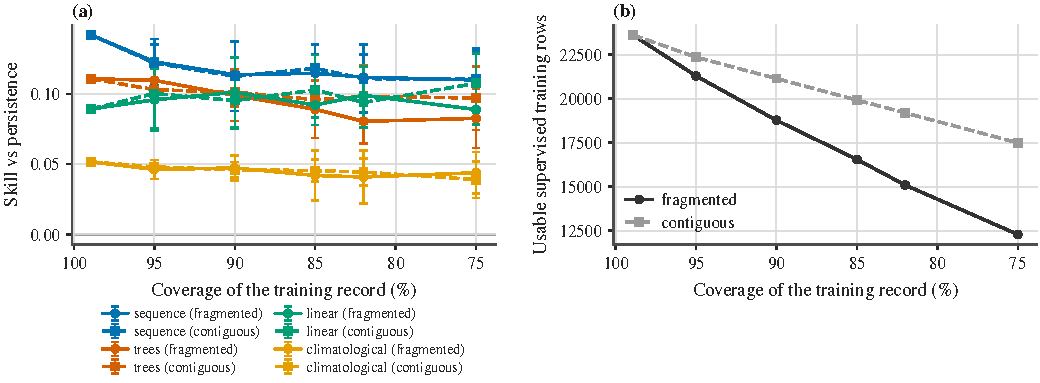
\includegraphics[width=\linewidth]{fig11_gap_injection.pdf}}
\caption{The gap injection experiment on the donor record at 24 hours. (a) Skill against
persistence by family, fragmented arm as circles and contiguous arm as squares, error bars
over ten injection seeds. (b) Usable supervised training rows under the two arms. At every
level the arms removed an identical number of observed hours, so the vertical distance in (b)
is created purely by arrangement.}
\label{fig:injection}
\end{figure*}

\subsection{Benchmark accuracy and its limits}

Table~\ref{tab:headline} reports the 24 hour horizon. The validation selected recurrent model,
a single layer GRU with 16{,}193 parameters over a 24 hour window, reaches an RMSE of 57.70
\ugm{} averaged over five seeds against 73.76 for persistence, a skill score of $+0.218$. The
best classical competitor is random forest at 58.50, and the paired test on the selected seed
rejects equality with a Holm adjusted $p$ of 0.037. Intervals are a moving block bootstrap
of 1{,}000 resamples, blocked at 24 hours because consecutive hourly errors are correlated.

That is the strongest reading the data support, and it is weaker than it looks. The 95 per
cent model confidence set retains five of the nine candidates, so the recurrent model, the
three tree ensembles and ridge are not separable at this horizon. The horizon is a choice
rather than a finding. Across the five horizons tested, LightGBM beats the sequence tier
significantly at 1 hour and at 12 hours, and the sequence tier wins significantly only at 24.
Any single horizon headline is therefore itself a selection.

The identity of the winner is also unstable. Re running the selection rule on 2{,}000 resamples
of the seed set returns the reported configuration 45 per cent of the time and ten distinct
candidates win at least once, yet the consequence is bounded, since selecting on validation
rather than on test costs only $+0.05$ \ugm{} here. We therefore make claims about tiers, not
about architectures.

\begin{table}[!t]
\caption{Test performance at the 24 hour horizon.}
\label{tab:headline}
\centering
\footnotesize
\sbox{\tablebox}{%
\begin{tabular}{l c c c c}
\toprule
\textbf{Model} & \textbf{RMSE} & \textbf{95\% CI} & \textbf{Skill} & \textbf{MCS} \\
\midrule
GRU (16{,}193 par.) & 57.24 & [52.38, 62.17] & $+0.218$ & yes \\
\midrule
Random forest       & 58.50 & [53.45, 63.49] & $+0.207$ & yes \\
\midrule
XGBoost             & 58.70 & [53.64, 63.73] & $+0.204$ & yes \\
\midrule
LightGBM            & 59.02 & [54.03, 64.19] & $+0.200$ & yes \\
\midrule
Ridge               & 59.37 & [54.30, 64.34] & $+0.195$ & yes \\
\midrule
Climatology         & 65.43 & [60.52, 70.45] & $+0.113$ & no \\
\midrule
Seasonal naive      & 73.76 & [67.77, 79.86] & $\phantom{+}0.000$ & no \\
\midrule
Persistence         & 73.76 & [67.77, 79.86] & $\phantom{+}0.000$ & no \\
\midrule
SARIMAX             & 81.36 & [74.83, 87.93] & $-0.103$ & no \\
\bottomrule
\end{tabular}}
\usebox{\tablebox}
\tablenote{RMSE in \ugm. The GRU row is the validation selected seed, whose
predictions enter the paired tests; the five seed mean is $57.70\pm0.44$.}
\end{table}

\subsection{The cross city contrast}

Running the identical pipeline on the Beijing record gives a rank correlation between the two
cities' method orderings of only $+0.20$, so a benchmark run on either city alone would
recommend a different method. The comparison is nevertheless uninformative about
fragmentation. First, the comparison city cannot support a ranking at all, because its own
confidence set retains nine of nine candidates, persistence included. Second, the observational
gradient runs the wrong way. The sequence tier ranks first on the more fragmented record and
third on the near complete one, the opposite of what a fragmentation account predicts, and the
pair also confounds fragmentation with a harder problem, a shorter evaluation period and a
seasonal transition. We report it rather than set it aside, and treat it as the reason to build
a counterfactual.

\subsection{The cost of arrangement at constant volume}

Fig.~\ref{fig:injection} shows the experiment, and panel (b) is the mechanism in one line. At
every coverage level the two arms have removed exactly the same number of observed hours, and
yet the fragmented arm retains several thousand fewer usable supervised rows, a deficit that
widens as the record degrades. Panel (a) shows what that costs. Each pair of a coverage level
and an injection seed gives one matched observation, so each family contributes 50 pairs. We
write the \emph{arm gap} for fragmented minus contiguous skill within such a pair, so a
negative value means fragmentation costs that family more than removing the same hours
contiguously. Table~\ref{tab:arm} reports the signed rank test, Holm corrected across
families. The sequence tier loses 0.0394 skill to arrangement alone, and it is not alone. The
climatological and tree families also move, and only the linear family is indistinguishable
from zero, so fragmentation is costly to most of the methods considered and most costly to the
one that reads windows.

\subsection{Replication across donor stations}

One record cannot distinguish a property of fragmentation from a property of a station, so
the experiment was repeated on two further stations of the same archive. We adopt a strict
replication rule, requiring the same sign and Holm significance on every donor.
Table~\ref{tab:arm} reports the outcome, an asterisk marking Holm significance within that
donor. Only the sequence tier replicates. The climatological
family is the reason more than one donor was run. On the first donor alone its penalty collapses
to $-0.096$ at the severest degradation, which read in isolation would have argued that
fragmentation degrades anything estimated from the record. It does not survive the other two
stations, so that collapse is a property of that station.

Significance against a family's own null on every donor is not, however, a contrast between
families. The stronger claim, that the sequence tier suffers \emph{most}, requires differencing
families within matched triples of coverage level, injection seed and donor. Under an
intersection union test, correct here because the claim is a conjunction, it fails. The
sequence tier separates from the linear and climatological families but not from the tree
ensembles, where the difference is $-0.0102$ with $p=0.15$. We therefore withhold the
comparative claim. The narrower one survives, that the sequence tier's penalty is the only one
appearing reliably across records and the largest in mean.

What does discriminate is the shape of the penalty in coverage. A cost flat in coverage is a
fixed toll, whereas one that steepens is a mechanism. Fitting one slope per injection seed and
donor, the sequence penalty steepens by 0.0226 per ten percentage points of coverage lost
while the tree penalty is flat and not significant. That is the shape the next subsection
predicts, and the pooled test averages it away.

\begin{table*}[!t]
\caption{Effect of arrangement at constant data volume.}
\label{tab:arm}
\centering
\footnotesize
\sbox{\tablebox}{%
\begin{tabular}{l r c c r r r c r c}
\toprule
& \multicolumn{3}{c}{\textbf{Pooled paired test}} & \multicolumn{4}{c}{\textbf{Per donor arm gap}} & \multicolumn{2}{c}{\textbf{Dose response}} \\
\cmidrule(lr){2-4}\cmidrule(lr){5-8}\cmidrule(lr){9-10}
\textbf{Family} & \textbf{Mean gap} & \textbf{95\% CI} & \textbf{$p$ (Holm)} & \textbf{Wanliu} & \textbf{Dingling} & \textbf{Dongsi} & \textbf{Replicates} & \textbf{Slope} & \textbf{$p$ (Holm)} \\
\midrule
Sequence       & $-0.0394$ & $[-0.0565,\,-0.0236]$ & $<0.0001$ & $-0.0394^{*}$ & $-0.0200^{*}$ & $-0.0273^{*}$ & \textbf{yes} & $-0.0226$ & $0.016$ \\
\midrule
Climatological & $-0.0357$ & $[-0.0609,\,-0.0138]$ & $0.0115$  & $-0.0357^{*}$ & $-0.0017$     & $-0.0206^{*}$ & no           & $-0.0247$ & $0.062$ \\
\midrule
Trees          & $-0.0263$ & $[-0.0393,\,-0.0125]$ & $0.0003$  & $-0.0263^{*}$ & $-0.0120$     & $-0.0179^{*}$ & no           & $-0.0052$ & $0.164$ \\
\midrule
Linear         & $-0.0016$ & $[-0.0081,\,+0.0047]$ & $0.9542$  & $-0.0016$     & $-0.0356^{*}$ & $-0.0225^{*}$ & no           & $-0.0173$ & $0.019$ \\
\bottomrule
\end{tabular}}
\usebox{\tablebox}
\tablenote{Fifty matched pairs per family per donor; representatives are fixed on
the undegraded record. Differencing families within matched triples does not
separate sequence from trees ($-0.0102$, $p=0.15$), so the comparative claim is
withheld.}
\end{table*}

\subsection{Mediation by the backward reach}

The account in \eqref{eq:radius} predicts something falsifiable. If the penalty is caused by
sterilised history rather than by lost hours, shortening the reach should shrink it. Because
the reach is set by configuration rather than inferred from a regression, the design needs no
ignorability assumption. The injection is deterministic in arm, coverage and seed and runs
before any feature is built, so the same degraded series appears at every reach and each draw is
a repeated measure.

The mediator moves first. Relative to the contiguous arm at an identical removed hour count,
the fragmented arm loses 8{,}056 usable training rows at $R=192$, 4{,}415 at $R=72$ and
3{,}220 at $R=48$. The penalty follows it, as Table~\ref{tab:mediation} shows, the sequence
gap falling from $-0.0394$ to $-0.0012$. Each test there is one sided and declared in advance,
because the mechanism predicts a single direction.

One confound must be bounded rather than argued away. A shorter reach scores more evaluation
hours, 4{,}806 against 3{,}813, so the two gaps are not measured on the same rows. Even if those
extra hours carried no arm difference whatever, the gap would shrink to 80 per cent of itself by
arithmetic alone, which accounts for 0.0079 of the observed change of 0.0383 and leaves 79 per
cent attributable to the reach. The falsification control holds too, since the linear family had
no penalty to mediate and shows no mediation.

\begin{table}[!t]
\caption{Arm gap at the configured reach against a quartered reach.}
\label{tab:mediation}
\centering
\footnotesize
\setlength{\tabcolsep}{3.5pt}
\begin{tabular}{l r r r r r}
\toprule
\textbf{Family} & \textbf{$R{=}192$} & \textbf{$R{=}48$} & \textbf{Change} & \textbf{Med.} & \textbf{$p$ (Holm)} \\
\midrule
Sequence       & $-0.0394$ & $-0.0012$ & $+0.0383$ & 97\,\% & $<0.0001$ \\
\midrule
Climatological & $-0.0357$ & $-0.0005$ & $+0.0351$ & 99\,\% & $0.0097$ \\
\midrule
Trees          & $-0.0263$ & $-0.0072$ & $+0.0191$ & 73\,\% & $0.0017$ \\
\midrule
Linear         & $-0.0016$ & $+0.0021$ & $+0.0037$ & ---    & $0.2605$ \\
\bottomrule
\end{tabular}
\end{table}

\subsection{A closed form for usable supervision}

If the radius is what a gap spends, the quantity of supervision a record can support should be
predictable from the record alone. Writing $U$ for usable rows, $O$ for observed hours and $k$
for distinct gaps,
\begin{equation}
U\approx O\exp\!\left(\beta_0-\alpha Rk/O\right),\;\; \alpha=0.1555,\; \beta_0=-0.1596 .
\label{eq:law}
\end{equation}
Fitted on the 101 cells of one donor grid at $R=192$, \eqref{eq:law} predicts 404 held out
cells at $R^2=0.982$ with a median absolute error of 3.5 per cent, as Fig.~\ref{fig:law}
shows. Those cells are two different extrapolations. Two hundred and two come from the other
stations at the same radius, asking whether the constants travel between records ($R^2$ of
0.970 and 0.983). The remaining 202 are the \emph{fitting} station rebuilt at $R=72$ and
$R=48$, asking whether $R$ is a factor of the form or a scale the constants absorbed ($R^2$ of
0.979 and 0.964). Scoring that second group at the fitted radius instead collapses the pooled
$R^2$ to 0.461, which is what the radius term carries.

The constant $\alpha$ is not free either. It should equal the share of gaps outliving the
short forward fill, which is 0.1418 across this record's 2{,}074 gaps with a 95 per cent
interval of $[0.1274, 0.1574]$. The fitted value falls inside that interval, so the constant
is the imputation policy rather than a fitted parameter. A near complete record is therefore not
a well supervised one. Amplification, being usable hours destroyed per hour missing, runs at 2.3
on the primary record and at 34.2, 14.0 and 10.4 on the three near complete stations, because it
follows the number of gaps and not their total length.

\begin{figure*}[!t]
\centerline{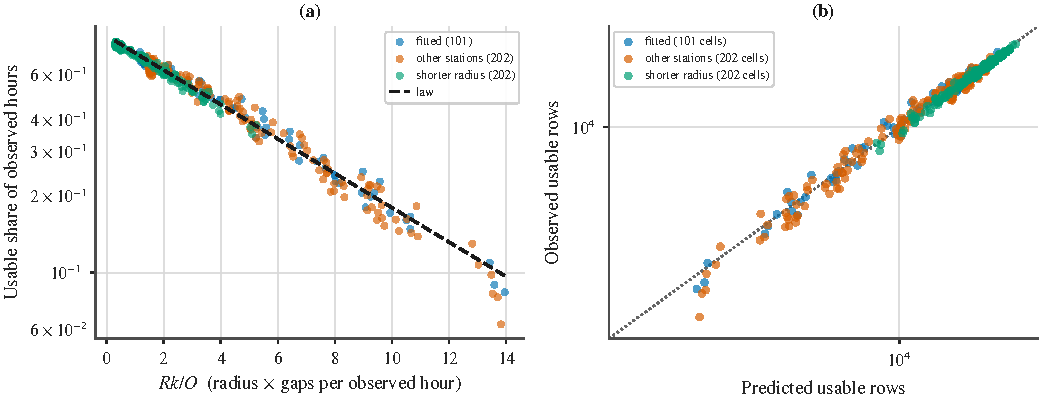
\includegraphics[width=\linewidth]{fig14_missingness_amplification.pdf}}
\caption{The amplification law of \eqref{eq:law}. (a) Usable share of observed hours against
$Rk/O$, fitted on 101 cells of one station's grid at $R=192$. (b) Predicted against observed
usable rows for all 505 cells. The held out sets are two distinct extrapolations, one across
stations at the fitted radius and one across radii on the fitting station.}
\label{fig:law}
\end{figure*}

\subsection{The price of the backward reach}

Anyone holding a record can price a reach exactly, with no fitted constants at all. A run of
length $l$ supports $\max(0,\,l-R)$ scored rows, so
\begin{equation}
U(R)=\sum_{\mathrm{runs}}\max(0,\,l-R),
\qquad
-\frac{\mathrm{d}U}{\mathrm{d}R}=\#\{l>R\} .
\label{eq:identity}
\end{equation}
One further hour of backward reach costs exactly the number of runs still longer than it.
Divided by $U/R$ it becomes an elasticity, the only form of the price comparable across records
of different sizes. Table~\ref{tab:avail} gives it. At the configured radius the primary record
pays 0.372 against the donor's 0.139, so a reach one per cent deeper costs it 2.7 times as large
a share of its supervision. The same table shows why coverage is the wrong summary statistic.
Hourly coverage runs 82.3 per cent on the primary record against 98.9 on the
donor, and yet availability runs 76.4 against 72.5, because the primary record's absences are
clustered into a few long outages while the near complete stations' are scattered. Coverage is
what a custodian reports. Availability is what a forecaster gets.

The trade was measured rather than assumed. Refitting every model at capped reaches and scoring
on the 9{,}083 hours every arm can serve, no capped arm beats the configured reach and none
loses to it, across 28 Holm corrected paired tests. Shortening the reach is not better at
forecasting. It is better at answering. Over a fixed universe in which an unanswered hour falls
back to persistence, capping at 24 hours raises availability from 83.5 to 97.6 per cent and is
worth $+0.0154$ median skill, $+0.0204$ for the best model.

Two qualifications keep this honest. The gain is not the rescue of catastrophic hours, because
the unserved hours are \emph{easier} than the served ones, persistence scoring 56.90 there
against 73.76. It is a model beating persistence over a large block of ordinary hours. The free
price also sizes the opportunity without promising the payoff, since the primary record recovers
48 per cent of its training rows against the donor's 9 per cent and yet gains less skill.
Availability, not rows, orders the two correctly.

\begin{table}[!t]
\caption{Availability and the price of the backward reach.}
\label{tab:avail}
\centering
\footnotesize
\begin{tabular}{l r r r r}
\toprule
& \multicolumn{2}{c}{\textbf{Availability}} & \textbf{Ampl.} & \textbf{Elast.} \\
\cmidrule(lr){2-3}
\textbf{Record} & \textbf{$R{=}192$} & \textbf{$R{=}48$} & \textbf{(\texttimes)} & \textbf{at 192} \\
\midrule
Dhaka             & 76.4\,\% & 87.2\,\% & 2.3  & 0.372 \\
\midrule
Beijing Wanliu    & 72.5\,\% & 85.5\,\% & 34.2 & 0.139 \\
\midrule
Beijing Dingling  & 64.4\,\% & 80.9\,\% & 14.0 & 0.213 \\
\midrule
Beijing Dongsi    & 64.3\,\% & 81.2\,\% & 10.4 & 0.168 \\
\bottomrule
\end{tabular}
\end{table}

\section{Discussion and Limitations}

The result that survives every check here is not a claim about architectures. It is that the
arrangement of absences is an experimental variable with a measurable effect on which method a
benchmark recommends, that the effect is carried by the backward reach a scored row requires,
and that the resulting loss of supervision is predictable from two counts a custodian already
holds. A benchmark reporting accuracy without availability reports a conditional quantity as
though it were unconditional.

Several limits are worth stating. The injection experiment runs at one horizon with one injected
gap length distribution, and its three donors are stations of a single archive covering one four
year window and one weather regime. That makes it a station robustness check, able to falsify a
station specific effect but not evidence of generality across cities. The comparative claim that
the sequence tier suffers most does not survive an intersection union test and is not made, and
the mediation result is established only on the record where the penalty was measured. The
target series comes from a single monitor, so results describe that site rather than Dhaka as a
whole. Ridge, disadvantaged by a logarithmic target with raw scale history, is a linear floor
rather than a tuned competitor. Inverting that logarithmic scale finally returns something
nearer a conditional median, so every model here underpredicts the largest episodes. The bias is
common to all of them, so between model comparisons remain valid.

\section{Conclusion}

Record fragmentation is not a preprocessing detail. Holding a record fixed and manipulating only
the arrangement of its absences costs the sequence tier 0.0394 skill at constant data volume,
and that is the only family whose loss replicates across three stations. The mechanism is the
backward reach a scored row demands. Quartering that reach removes 97 per cent of the penalty,
and the supervision a record can support follows a closed form in observed hours, gap count and
reach that predicts 404 held out cells at $R^2=0.982$. Price the reach before choosing it,
because here the configured reach bought no accuracy and cost fourteen points of the hours a
forecast could be issued at all.

\begin{thebibliography}{00}
\bibitem{who2021} World Health Organization, \emph{WHO Global Air Quality Guidelines}. Geneva, Switzerland: WHO, 2021.
\bibitem{li2017lstm} X. Li et al., ``Long short-term memory neural network for air pollutant concentration predictions,'' \emph{Environ. Pollut.}, vol. 231, pt. 1, pp. 997--1004, 2017.
\bibitem{karnati2025} H. Karnati et al., ``Comprehensive analysis of various imputation and forecasting models for predicting PM2.5 pollutant in Delhi,'' \emph{Neural Comput. Appl.}, vol. 37, pp. 11441--11458, 2025.
\bibitem{che2018grud} Z. Che, S. Purushotham, K. Cho, D. Sontag, and Y. Liu, ``Recurrent neural networks for multivariate time series with missing values,'' \emph{Sci. Rep.}, vol. 8, art. 6085, 2018.
\bibitem{hochreiter1997lstm} S. Hochreiter and J. Schmidhuber, ``Long short-term memory,'' \emph{Neural Comput.}, vol. 9, no. 8, pp. 1735--1780, 1997.
\bibitem{cho2014gru} K. Cho et al., ``Learning phrase representations using RNN encoder-decoder for statistical machine translation,'' in \emph{Proc. EMNLP}, 2014, pp. 1724--1734.
\bibitem{zeng2023dlinear} A. Zeng, M. Chen, L. Zhang, and Q. Xu, ``Are transformers effective for time series forecasting?,'' in \emph{Proc. AAAI}, vol. 37, no. 9, 2023, pp. 11121--11128.
\bibitem{rubin1976} D. B. Rubin, ``Inference and missing data,'' \emph{Biometrika}, vol. 63, no. 3, pp. 581--592, 1976.
\bibitem{diebold1995} F. X. Diebold and R. S. Mariano, ``Comparing predictive accuracy,'' \emph{J. Bus. Econ. Statist.}, vol. 13, no. 3, pp. 253--263, 1995.
\bibitem{holm1979} S. Holm, ``A simple sequentially rejective multiple test procedure,'' \emph{Scand. J. Statist.}, vol. 6, no. 2, pp. 65--70, 1979.
\bibitem{hansen2011mcs} P. R. Hansen, A. Lunde, and J. M. Nason, ``The model confidence set,'' \emph{Econometrica}, vol. 79, no. 2, pp. 453--497, 2011.
\bibitem{kunsch1989} H. R. K\"{u}nsch, ``The jackknife and the bootstrap for general stationary observations,'' \emph{Ann. Statist.}, vol. 17, no. 3, pp. 1217--1241, 1989.
\bibitem{zhang2017beijing} S. Zhang et al., ``Cautionary tales on air-quality improvement in Beijing,'' \emph{Proc. Roy. Soc. A}, vol. 473, no. 2205, art. 20170457, 2017.
\bibitem{openaq} OpenAQ. (2025). \emph{OpenAQ Open Air Quality Data Archive}. [Online]. Available: \url{https://openaq.org}
\bibitem{nasapower} NASA Langley Research Center. (2025). \emph{POWER Hourly Point Data}. [Online]. Available: \url{https://power.larc.nasa.gov}
\bibitem{doe2025} Department of Environment, Bangladesh, \emph{Ambient Air Quality in Bangladesh (2018--2023)}. Dhaka, 2025.
\bibitem{schwartz2020} R. Schwartz, J. Dodge, N. A. Smith, and O. Etzioni, ``Green AI,'' \emph{Commun. ACM}, vol. 63, no. 12, pp. 54--63, 2020.
\bibitem{bergmeir2012} C. Bergmeir and J. M. Ben\'{i}tez, ``On the use of cross-validation for time series predictor evaluation,'' \emph{Inf. Sci.}, vol. 191, pp. 192--213, 2012.
\end{thebibliography}

\end{document}
